% ============================================================
\chapter{Multi-Cohort Integration and Joint Modelling}
\label{chap:multi_cohort_integration}
% ============================================================

% ------------------------------------------------------------
\section{Rationale for Multi-Cohort Integration}
% ------------------------------------------------------------

The single-cohort analyses presented in Chapters~\ref{chap:feature_selection}
and~\ref{chap:model_training_evaluation} established that Normal--Adjacent methylation differences
are detectable within each dataset independently, yet the cross-cohort transfer
experiments of Section~\ref{sec:cross_dataset} revealed a fundamental obstacle:
the discriminative axes identified in isolation are not mutually transferable,
and in one direction performance inverts below chance level.
This failure is attributable to two concurrent factors.
First, the three cohorts originate from different Illumina platforms
(HumanMethylation450K for GSE69914, MethylationEPIC for GSE225845 and GSE287331),
introducing systematic probe-design and coverage differences.
Second, and more critically, the uncorrected pool is dominated by inter-study
variance that absorbs the comparatively subtle biological signal of early
epigenetic drift.
The present chapter addresses both obstacles simultaneously by constructing a
unified analytical framework in which all three cohorts are harmonised,
jointly preprocessed, and modelled as a single integrated dataset.
The objective is not external validation --- which would require a fully held-out
study --- but the assessment of signal stability under controlled multi-cohort
pooling, where biological heterogeneity and platform variability coexist within
a single analytical setting.
A discriminative panel that retains predictive ability in this pooled regime
can be considered cohort-invariant to a meaningful degree, encoding shared
biological processes rather than study-specific artefacts.



% ------------------------------------------------------------
\section{Multi-Cohort Integration Framework}
% ------------------------------------------------------------
This section describes the sequence of operations applied to construct the harmonised multi-cohort representation. The pipeline proceeds in three ordered steps --- feature-space alignment, absolute deviation transformation, and batch harmonisation --- each designed to address a specific obstacle to cross-cohort integration while maintaining strict separation between training and test data.
\subsection{Construction of a Shared CpG Feature Space}
Integration begins with the construction of a shared feature space.
After applying the per-dataset preprocessing pipelines described in
Chapter~\ref{chap:data_preprocessing} --- including technical probe filtering,
sex-chromosome exclusion, and manifest-based annotation validation ---
the three cleaned CpG sets are intersected.
The resulting common space comprises $215{,}919$ autosomal CpGs consistently
retained across all three platforms after filtering, forming the backbone for
all downstream operations.
Before any transformation or modelling step, a single stratified train--test
split is performed on the aggregated pool of 587 samples.
Stratification is carried out jointly on dataset identity and tissue label,
yielding a training set of 410 samples and a test set of 177 samples,
with class and cohort proportions preserved in both partitions.
This split is fixed for the entire chapter; the test set is never consulted
during preprocessing, transformation, feature selection, or model training,
guaranteeing a strictly leakage-free evaluation.

\subsection{Absolute Deviation Transformation}

A key challenge identified in Chapter~\ref{chap:model_training_evaluation} is the directional
inconsistency of methylation drift across cohorts: the sign of
$\Delta M$ (Adjacent $-$ Normal) is not uniform, with GSE287331 exhibiting a
predominantly opposite direction relative to the two EPIC cohorts
(Figure~\ref{fig:deltam_scatter}).
Training a standard linear classifier on signed $M$-values under these conditions
forces the model to learn contradictory decision boundaries, suppressing
cohort-invariant signal.
To resolve this, each sample is transformed into its absolute deviation from the
within-cohort Normal mean before pooling.
Formally, for each dataset $d$ and each CpG $j$, the transformed feature is:
\begin{equation}
  \tilde{x}_{ij} = \bigl|\, x_{ij} - \bar{\mu}^{(d)}_{\mathrm{Normal},j} \,\bigr|,
\end{equation}
where $\bar{\mu}^{(d)}_{\mathrm{Normal},j}$ is the mean $\beta$-value of Normal
samples in the training partition of cohort $d$.
This mean is estimated exclusively on the training split of each dataset and
applied without re-estimation to the corresponding test samples, preserving the
leakage-free design.
Under the field cancerisation hypothesis, Adjacent tissue is expected to deviate
more from the Normal reference than Normal tissue itself, regardless of drift
direction; the absolute deviation representation makes this deviation comparable
across cohorts with opposite drift orientations.

\subsection{Batch Harmonisation via NeuroCombat}
\label{sec:neurocombat}

Even after the absolute deviation transformation, residual inter-study variance
persists in the pooled training matrix, reflecting differences in sample
preparation, technical processing, and cohort-specific biological composition.
To remove these additive and multiplicative batch effects while preserving
biologically relevant covariance, the NeuroCombat harmonisation
framework~\cite{fortin2018neurocombat} is applied to the pooled training set of 410 samples.
NeuroCombat models each feature as:
\begin{equation}
Y_{ijd} = \alpha_j + X\beta_j + \gamma_{jd} + \delta_{jd}\varepsilon_{ijd},
\end{equation}
where $\gamma_{jd}$ and $\delta_{jd}$ are the additive and multiplicative batch
parameters for cohort $d$, estimated via empirical Bayes shrinkage.
The biological covariate matrix $X$ includes tissue label (Normal vs.\ Adjacent)
as a categorical variable and chronological age as a continuous covariate.
Age is included because DNA methylation varies with age in a systematic,
locus-specific manner~\cite{Horvath2013}; including it as a protected covariate
prevents ComBat from absorbing age-related methylation variance into the batch
correction.
The chronological age used here is derived from the metadata of each cohort;
its estimation and quality assessment are detailed in Appendix~\ref{app:age_estimation}.
ComBat parameters are estimated exclusively on the training pool.
The resulting estimates are then applied to the test set via
\texttt{neuroCombatFromTraining}, which applies the pre-fitted transformation
without re-estimating any parameters --- a strict zero-leakage design.


% ------------------------------------------------------------
\section{Batch Harmonisation Diagnostics}
% ------------------------------------------------------------

\begin{figure}[t]
\centering
\begin{subfigure}[b]{0.48\textwidth}
  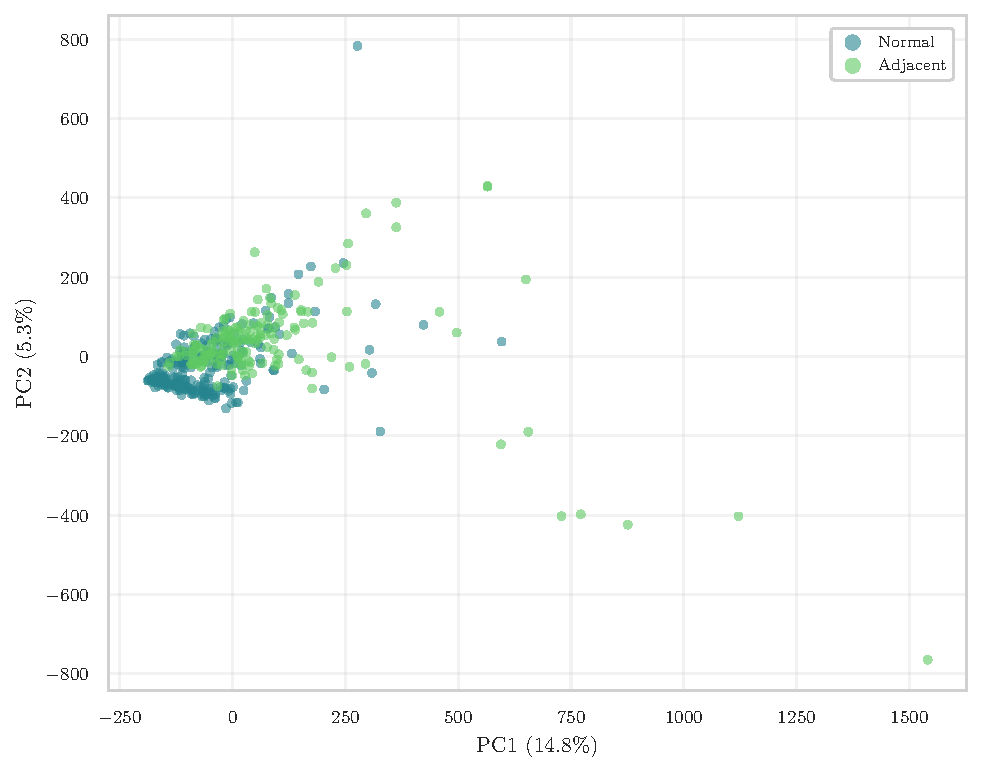
\includegraphics[width=\textwidth]{images/cap7/plot_pca_precombat_by_label.pdf}
  \caption{Coloured by tissue label.}
\end{subfigure}
\hfill
\begin{subfigure}[b]{0.48\textwidth}
  
\includegraphics[width=\textwidth]{images/cap7/plot_pca_precombat_by_dataset.pdf}
  \caption{Coloured by cohort of origin.}
\end{subfigure}
\caption{PCA of the pooled training set \emph{prior} to NeuroCombat
  (PC1\,=\,14.8\%, PC2\,=\,5.3\%). Batch variance dominates PC1;
  no tissue-label separation is visible.}
\label{fig:pca_pre_combat}
\end{figure}

\begin{figure}[t]
\centering
\begin{subfigure}[b]{0.48\textwidth}
  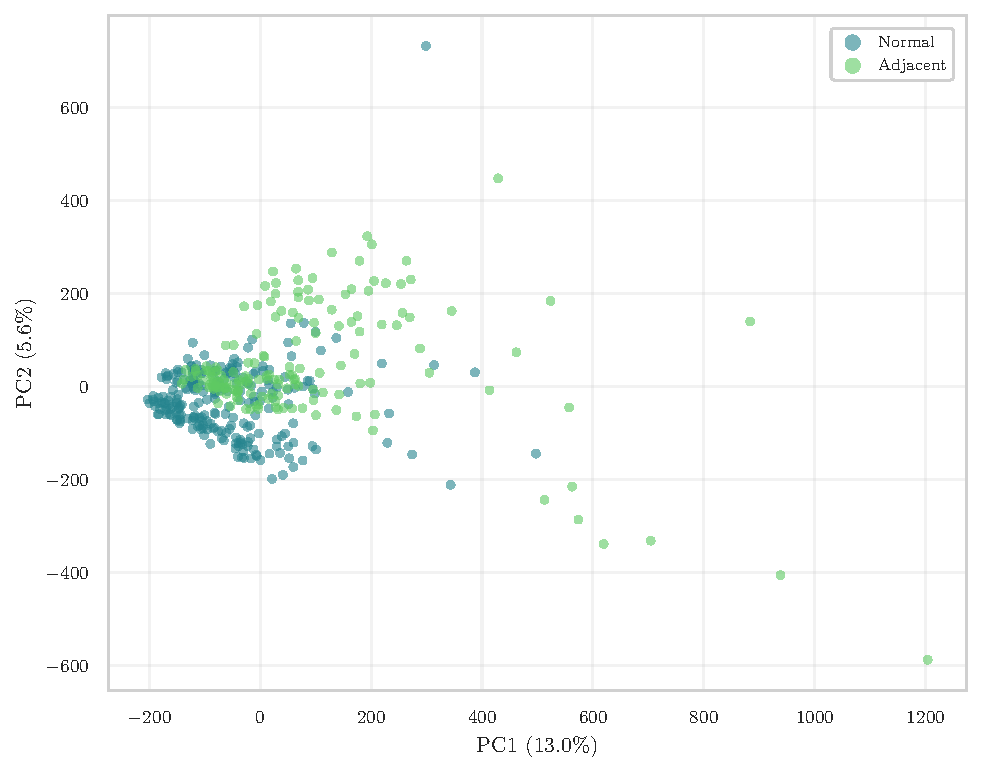
\includegraphics[width=\textwidth]{images/cap7/plot_pca_postcombat_by_label.pdf}
  \caption{Coloured by tissue label.}
\end{subfigure}
\hfill
\begin{subfigure}[b]{0.48\textwidth}
  
\includegraphics[width=\textwidth]{images/cap7/plot_pca_postcombat_by_dataset.pdf}
  \caption{Coloured by cohort of origin.}
\end{subfigure}
\caption{PCA of the pooled training set \emph{after} NeuroCombat
  (PC1\,=\,13.0\%, PC2\,=\,5.6\%). Cohort-driven elongation is substantially
  reduced; a partial Normal--Adjacent separation emerges along PC1.}
\label{fig:pca_post_combat}
\end{figure}

The effectiveness of the harmonisation pipeline is assessed through principal
component analysis of the pooled training matrix, computed before and after
ComBat correction.
Before harmonisation (Figure~\ref{fig:pca_pre_combat}), the first principal
component captures 14.8\% of variance and is dominated by cohort identity:
GSE287331 samples form an elongated scatter extending along PC1, consistent
with the strong platform-specific signal documented in earlier chapters.
When the same projection is coloured by tissue label, no Normal--Adjacent
separation is discernible, confirming that the biological axis is masked by
batch-driven variance.
After NeuroCombat correction (Figure~\ref{fig:pca_post_combat}), the
cohort-driven elongation is substantially reduced.
The three datasets mix more uniformly in the PC1--PC2 plane, and a partial
separation by tissue label begins to emerge along PC1 (13.0\%).
The modest but consistent restructuring of the variance landscape confirms
that ComBat has attenuated the dominant inter-study component while exposing
the underlying biological signal.



% ------------------------------------------------------------
\section{Feature Selection and Predictive Modelling}
% ------------------------------------------------------------
This section describes the feature selection and classification pipeline applied to the harmonised pooled matrix, and reports the resulting predictive performance on the held-out test set. The pipeline mirrors the intra-dataset procedure of Chapter~\ref{chap:feature_selection} and Chapter~\ref{chap:model_training_evaluation}, here adapted to the multi-cohort setting.

\subsection{Feature Selection on the Harmonised Pool}

Following harmonisation, the stability-driven feature selection procedure
introduced in Chapter~\ref{chap:feature_selection} is applied to the pooled
training matrix.
Edgar $\beta$-variability filtering reduces the initial 215{,}919 CpGs to
106{,}289, and subsequent $\beta \rightarrow M$ transformation with
variance-based pruning (bottom 2\% SD removed) yields a working set of
\num{104163} features.
Biological weighting assigns higher priority to CpG island and promoter-proximal
loci, and repeated stratified K-fold stability ranking ($K=5$, $R=10$,
50 splits total) with $S_{\mathrm{dir}} \geq 0.75$ selects 15{,}000 candidate
CpGs, with Spearman $\rho(\mathrm{score},|\Delta M|) = -0.78$ confirming
strong alignment between ranking and effect size.
Region anchoring on CpG islands identifies 1{,}165 stable regions
and produces Pool~A of 2{,}740 anchored CpGs.
Correlation-based redundancy pruning ($|r| \geq 0.85$) and genomic
diversification with chromosomal (max 8\% per chromosome) and spatial
constraints (max 15 CpGs per 500\,kb window, zero violations) yield the final
panel of 5{,}000 CpGs.


\subsection{Linear SVM Training and Panel Compression}

A linear SVM with StandardScaler preprocessing is trained on the 5{,}000-CpG.
Five-fold cross-validation over $C \in \{0.001, 0.01, 0.1, 1.0, 10.0\}$ yields
a stable CV AUC of $0.973 \pm 0.021$ across all regularisation values;
$C = 0.1$ is selected.
The learned coefficient vector is fed into the MILP knapsack formulation
(Section~\ref{sec:knapsack}), which compresses the panel to 50 biologically
constrained CpGs under joint optimisation of discriminative performance and
COSMIC breast-cancer gene enrichment ($\mu = 1.0$, $w_{\mathrm{COSMIC}} = 0.7$,
selected via knee-point analysis on the AUC--enrichment sweep).
The knapsack increases the number of COSMIC breast-cancer genes from 11
(at $\mu=0$, pure performance) to 18, the number of CpG island loci
from 39 to 42, and the number of promoter-proximal loci from 29 to 32,
while mapping to 42 unique genes.

\subsection{Predictive Performance}

\begin{table}[t]
\centering
\scriptsize
\caption{Performance of the 5{,}000-CpG SVM and the 50-CpG knapsack panel on the pooled test set, with per-cohort AUC breakdown.}
\label{tab:pooled_results}
\begin{tabular}{l c c c c c}
\toprule
Model & AUC & BACC & AUC GSE69914 & AUC GSE225845 & AUC GSE287331 \\
\midrule
SVM 5{,}000 CpG & 0.944 & 0.849 & 0.528 & 0.951 & 1.000 \\
SVM 50 CpG knapsack & 0.902 & 0.799 & 0.487 & 0.827 & 1.000 \\
\bottomrule
\end{tabular}
\end{table}

\begin{figure}[t]
\centering
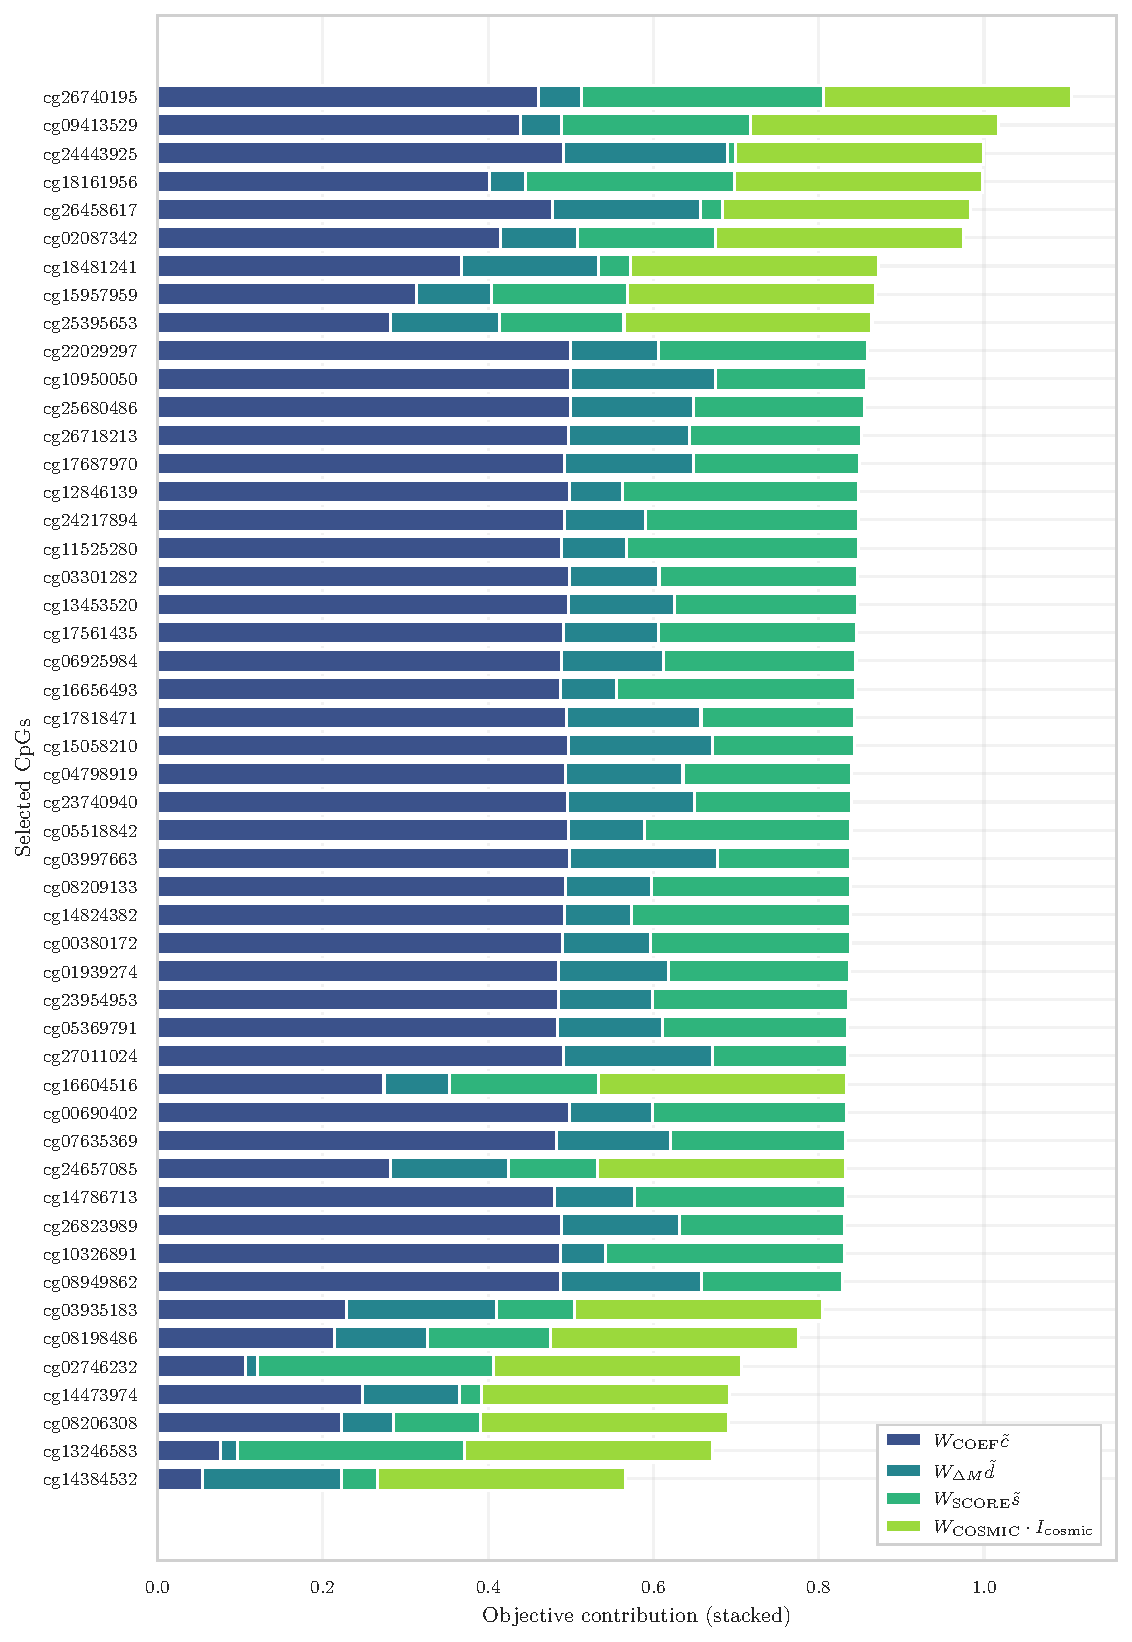
\includegraphics[width=0.65\textwidth]
  {images/cap7/knapsack_selected_contributions_stacked.pdf}
\caption{Component-wise decomposition of the MILP objective for the 50-CpG
  multi-cohort panel.}
\label{fig:cap7_knapsack}
\end{figure}




Performance on the pooled test set (177 samples: 104 Normal, 73 Adjacent)
is reported in Table~\ref{tab:pooled_results}.
The per-cohort breakdown reveals a heterogeneous picture.
GSE287331 achieves perfect separation at both panel sizes,
consistent with the strong intra-dataset signal documented in
Chapter~\ref{chap:model_training_evaluation}.
GSE225845 retains good discriminative ability at 50 CpGs,
representing a moderate but acceptable degradation from the 5{,}000-CpG
upper bound.
GSE69914, however, remains near chance level even with
the full panel, mirroring the low intra-dataset signal observed in isolation
and suggesting that the HM450K cohort contributes structural diversity to the
panel without contributing proportional discriminative power. 


% ------------------------------------------------------------
\section{Biological Interpretation of the 50-CpG Panel}
% ------------------------------------------------------------

\begin{figure}[t]
\centering
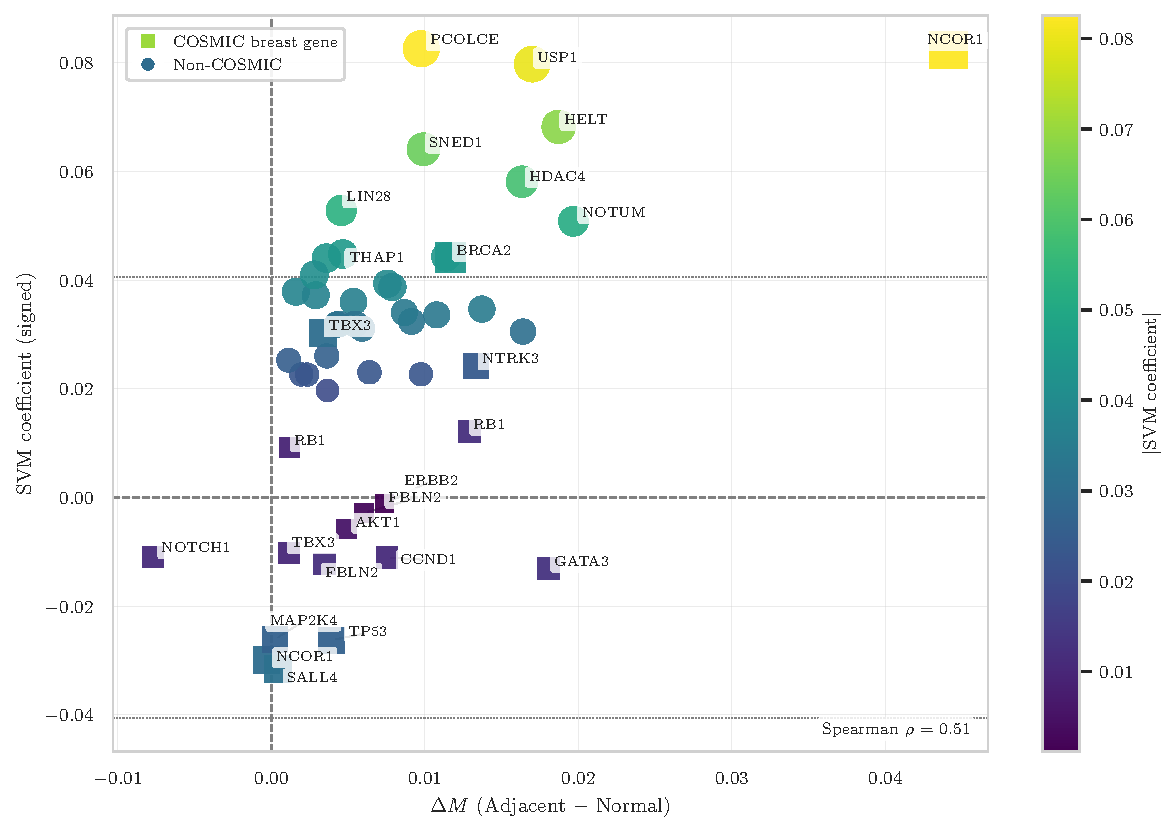
\includegraphics[width=0.55\textwidth]
  {images/cap7/volcano_50cpg_multicohort_signedcoef_shapes.pdf}
\caption{SVM coefficient (signed) versus $\Delta M$ (Adjacent $-$ Normal,
  absolute-deviation space) for the 50 selected loci.
  Spearman $\rho = 0.51$ indicates moderate concordance between discriminative
  weight and deviation magnitude.}
\label{fig:cap7_volcano}
\end{figure}

The 50 selected CpGs map to 49 unique genes via Illumina manifest
annotation (50/50 CpGs annotated).
Of these, 18 overlap with the COSMIC Cancer Gene Census breast-cancer subset
(44 genes total), compared to 11 in the unconstrained baseline ($\mu = 0$),
demonstrating the effectiveness of the knapsack biological penalty.

The volcano plot (Figure~\ref{fig:cap7_volcano}) shows the relationship between
SVM discriminative weight and deviation magnitude for each of the 50 loci.
COSMIC breast-cancer genes span the full range of coefficient magnitudes and
both directions of the signed axis, consistent with the heterogeneous roles of
these genes in epigenetic field reprogramming.
Among the previously characterised COSMIC loci, notable examples include
TBX3 (hypomethylated, promotes invasion by bypassing senescence~\cite{fillmore2010tbx3}),
GATA3 (master regulator of luminal identity~\cite{asselin2007gata3}),
RB1 (G1/S checkpoint tumour suppressor~\cite{cancer2012comprehensive}),
NOTCH1 (developmental signalling, discussed in Section~\ref{sec:results_gse225845}),
NCOR1 (transcriptional co-repressor, discussed in Section~\ref{sec:results_gse225845}),
BRCA2 (DNA repair, discussed in Sections~\ref{sec:results_gse69914}--\ref{sec:results_gse287331}),
TP53, GATA3, AKT1, and SALL4 (discussed in respective single-cohort sections).
Three COSMIC loci appear in the multi-cohort panel for the first time and warrant
brief commentary.
HDAC4 (class\,IIa histone deacetylase): a transcriptional co-repressor that
suppresses CDK inhibitors including p21 and promotes cell-cycle progression;
its overexpression has been linked to invasion and angiogenesis in multiple
solid tumours through VEGF--HIF-1$\alpha$ signalling~\cite{DiGiorgio2023}.
NTRK3 (neurotrophic tyrosine kinase receptor 3): the kinase domain partner in
the ETV6--NTRK3 fusion oncogene that is the defining genetic event of secretory
breast carcinoma, constitutively activating RAS--MAPK and PI3K--AKT
pathways~\cite{tognon2002etv6}.
LIN28B (RNA-binding protein): an oncogenic suppressor of the let-7
microRNA family that derepresses MYC, RAS, and HMGA2; overexpressed in
triple-negative breast cancer and associated with poor differentiation and
advanced disease stage~\cite{Piskounova2011,Xie2014}.
The Spearman $\rho = 0.51$ between signed coefficient and $\Delta M$ indicates
moderate but imperfect concordance, reflecting the contribution of the knapsack
biological penalty terms in selecting loci beyond pure effect size.
The panel reflects the multifactorial nature of epigenetic field defects: it spans tumour suppressors (RB1, TP53), chromatin regulators (HDAC4, NCOR1), developmental transcription factors (TBX3, SALL4), signalling components (NOTCH1, NTRK3, AKT1), and an RNA-binding oncogene (LIN28B).
The panel reflects the multifactorial nature of epigenetic field defects:
it spans tumour suppressors (RB1, TP53), chromatin regulators (HDAC4, NCOR1),
developmental transcription factors (TBX3, SALL4), signalling components
(NOTCH1, NTRK3, AKT1), and an RNA-binding oncogene (LIN28B).
The inclusion of 18 COSMIC breast-cancer genes --- compared to 11 in the
unconstrained $\mu = 0$ baseline --- demonstrates that the knapsack constraints
are effective in directing the panel towards biologically interpretable loci
without a commensurate loss of discriminative performance.

% ------------------------------------------------------------
\section{Cross-Cohort Epigenetic Drift}
% ------------------------------------------------

The multi-cohort integration framework presented in this chapter demonstrates
that early epigenetic drift in breast tissue encodes a cohort-invariant signal,
accessible once inter-study batch effects and directional inconsistencies are
addressed.
The absolute deviation transformation resolves the polarity problem identified
in Chapter~\ref{chap:model_training_evaluation} by recasting the classification problem in
terms of deviation magnitude from the Normal reference.
NeuroCombat harmonisation then removes residual platform-specific variance,
as confirmed by the restructuring of the PCA landscape
(Figures~\ref{fig:pca_pre_combat}--\ref{fig:pca_post_combat}).
Stability-based feature selection on the harmonised pool identifies loci that
are consistently informative across heterogeneous study conditions, and the
MILP knapsack produces a compact, biologically grounded 50-CpG panel
(AUC\,=\,0.902, BACC\,=\,0.799 on the pooled test set) mapping to 18 COSMIC
breast-cancer genes at 100-fold compression.
The residual weakness on GSE69914 reflects a genuine biological signal
limitation rather than a methodological failure: the Normal--Adjacent contrast
in this HM450K cohort is inherently subtler, as documented in the
intra-dataset analyses, and the harmonised multi-cohort framework cannot
recover signal that is absent at source.
The strong performance on GSE287331 and GSE225845, spanning two independent
EPIC studies, provides meaningful evidence that the selected panel captures a
shared epigenetic signature of field cancerisation in breast tissue.